\subsection{The \moc{THM:} module}\label{sect:thm}

\vskip 0.2cm

The \moc{THM:} module is a simplified thermal-hydraulics module where the
reactor is represented as a collection of independent channels with no
cross-flow between them. Each channel is represented using 1D convection
equations along the channel and 1D cylindrical equations for a single pin cell.
A two-fluid homogeneous model is used. The \moc{THM:} module is built around {\sl freesteam},
an open source implementation of IAPWS-IF97 steam tables for light water.\cite{freesteam}.

\vskip 0.08cm

The simplified model used in  \moc{THM:} is based on the work of M. F. Fehri for CANDU clusters\cite{fehri} and P. Gallet
for PWR assemblies\cite{gallet}. The \moc{THM:} module works both in steady-state and in transient conditions and includes
a subcooled flow boiling model based on the {\sl Bowring} correlation\cite{bowring} or on the {\sl Saha-Zuber}
correlation\cite{saha-zuber} for computing the temperature subcooling at the onset of fully developed boiling (OFDB).

\vskip 0.08cm

The 1D thermal-hydraulics equations are solved in each channel as a fonction of two
{\sl fixed} inlet conditions for the coolant velocity and temperature and one {\sl fixed} outlet condition for the pressure.

\vskip 0.1cm

\noindent
The \moc{THM:} module specification is:

\begin{DataStructure}{Structure \moc{THM:}}
\dusa{THERMO} \dusa{MAPFL} \moc{:=} \moc{THM:}
$[$ \dusa{THERMO} $]$ \dusa{MAPFL} \moc{::} \dstr{descthm}
\end{DataStructure}

\noindent where

\begin{ListeDeDescription}{mmmmmmmm}

\item[\dusa{THERMO}] \texttt{character*12} name of the \dds{thermo}
object that will be created or updated by the \moc{THM:} module. Object \dds{thermo}
contains thermal-hydraulics information set or computed by \moc{THM:} in transient or in
permanent conditions such as the distribution of the enthalpy, the pressure, the velocity,
the density and the temperatures of the coolant for all the channels in the geometry. It also contains all the values of the fuel temperatures in transient or in permanent conditions according to the discretisation chosen for the fuel rods.

\item[\dusa{MAPFL}] \texttt{character*12} name of the \dds{map} 
object containing fuel regions description and local parameter informations.

\item[\dstr{descthm}] structure describing the input data to the \moc{THM:} module. 

\end{ListeDeDescription}

\vskip 0.2cm

\subsubsection{Input data to the \moc{THM:} module}\label{sect:thmstr}

\begin{DataStructure}{Structure \dstr{descthm}}
$[$ \moc{EDIT} \dusa{iprint} $]$ \\
$[$ \moc{FLUID} $\{$ \moc{H2O} $|$ \moc{D2O} $|$ \moc{SALT} \dusa{sname} \dusa{scomp} $\}~]$ \\
$[$ \moc{RELAX} \dusa{relax} $]$ \\
$[$ \moc{TIME} \dusa{time} $[$ \dusa{timestep} $]~]$ \\
$[$ \moc{FPUISS} \dusa{fract} $]~[$ \moc{CRITFL} \dusa{cflux} $]$ \\
\moc{INLET} \dusa{poutlet} \dusa{tinlet} \\
$\{$ \moc{CWSECT} \dusa{sect} \dusa{flow} $|$ \moc{INLET-Q} \dusa{sect} \dusa{qfluid} $|$ \moc{SPEED} \dusa{velocity} $\}$ \\
$\{$ \moc{ASSMB} $\{$ \dusa{nbf} $|$ \moc{CHAN} (\dusa{nbf}(i), i = 1, \dusa{nch} ) $\}~\{$ \dusa{nbg} $|$ \moc{CHAN} (\dusa{nbg}(i), i = 1, \dusa{nch} ) $\}$ \\
~~~$|$ \moc{CLUSTER} \dusa{pitch} $\{$ \dusa{nbf} $|$ \moc{CHAN} (\dusa{nbf}(i), i = 1, \dusa{nch} ) $\}~\}$ \\
\moc{RADIUS} \dusa{r1} \dusa{r2} \dusa{r3} \dusa{r4} \\
$[$ \moc{POROS} \dusa{poros} $]~[$ \moc{PUFR} $\{$ \dusa{pufr} $|$ \moc{CHAN} (\dusa{pufr}(i), i = 1, \dusa{nch} ) $\}~]$ \\
$[$ \moc{CONDF} \dusa{ncond} (\dusa{kcond}(k),k=0,\dusa{ncond}) $[$ \moc{INV} \dusa{inv} \dusa{ref} $]$ \dusa{unit} $]$ \\
$[$ \moc{F-RUG} \dusa{epsr} $]~[$ \moc{THETA} \dusa{theta} $]$ \\
$[$ \moc{CONDC} \dusa{ncond} (\dusa{kcond}(k),k=0,\dusa{ncond}) \dusa{unit} $]$ \\
$[$ \moc{HGAP} \dusa{hgap} $]~[$ \moc{HCONV} \dusa{hconv} $]~[$ \moc{TEFF} \dusa{wteff} $]$ \\
$[$ \moc{CONV} \dusa{maxit1} \dusa{maxit2} \dusa{maxit3} \dusa{ermaxt} \dusa{ermaxc} $]$ \\
$[$ \moc{RODMESH} \dusa{nb1} \dusa{nb2} $]$ \\
$[$ \moc{FORCEAVE} $]$ \\
$[~\{$ \moc{MONO} $|$ \moc{BOWR} $|$ \moc{SAHA} $\}~]$ \\
$[$ \moc{RAD-PROF} $[[$ \dusa{rprad} \dusa{fprad} $]]~]$ \\
$[$ \moc{POWER-LAW} \dusa{tpow} \dusa{ntime} (\dusa{t}(i) \dusa{pow}(i),i=1,\dusa{ntime}) $]$ \\
$[[$ \moc{SET-PARAM} \dusa{PNAME} \dusa{pvalue} $]]$ \\
$[$ \moc{PICK}  {\tt >>} \dusa{ratio} {\tt <<} $]$ \\
;
\end{DataStructure}

\noindent where
\begin{ListeDeDescription}{mmmmmmmm}

\item[\moc{EDIT}] keyword used to set \dusa{iprint}.

\item[\dusa{iprint}] integer index used to control the printing on screen:
= 0 for no print; = 1 for minimum printing; larger values produce
increasing amounts of output.

\item[\moc{FLUID}] keyword used to set the fluid type. By default, light water (H$_2$O) is used.

\item[\moc{H2O}] use light water (H$_2$O).

\item[\moc{D2O}] use heavy water (D$_2$O).

\item[\moc{SALT}] use molted salt.

\item[\dusa{sname}] molted salt formula.

\item[\dusa{scomp}] molted salt composition.

\item[\moc{RELAX}] keyword used to set the relaxation parameter \dusa{relax}.

\item[\dusa{relax}] relaxation parameter selected in the interval $0<$\dusa{relax}$\le 1$ and used to update
the fuel (average and surface) temperature, coolant temperature and coolant density. The updated value is taken equal to
$(1-$\dusa{relax}$)$ times the previous iteration value plus \dusa{relax} times the actual iteration value. The default
value is \dusa{relax}$=1$.

\item[\moc{TIME}] keyword used to specify the type of calculation (steady-state or transient) performed by the \moc{THM:} module and the temporal parameters. By default, a steady-state calculation is performed.
\item[\dusa{time}] real value of time in second. Equal to the current time in case of steady-state calculation. Equal to the time at beginning-of-step in
case of transient calculation. The default value is 0.0.
\item[\dusa{timestep}] real value (in second) set to the time step in case of a transient calculation. A steady-state/transient calculation is assumed
depending if this value is not given/is given. 

\item[\moc{FPUISS}] keyword used to specify the fraction of the power released in fuel. The remaining
fraction is assumed to be released in coolant. The default value is 0.974.

\item[\dusa{fract}] real value set to the fraction ($f$). Power densities released in coolant and
fuel are computed as
\begin{eqnarray*}
Q_{\rm cool} \negthinspace\negthinspace &=& \negthinspace\negthinspace (1-f)\, {V_{\rm cool}+V_{\rm fuel} \over V_{\rm cool}} \, {P_{\rm mesh} \over
V_{\rm mesh}} \\
Q_{\rm fuel} \negthinspace\negthinspace &=& \negthinspace\negthinspace f\, {V_{\rm cool}+V_{\rm fuel} \over V_{\rm fuel}} \, {P_{\rm mesh} \over
V_{\rm mesh}}
\end{eqnarray*}
\noindent where $V_{\rm cool}$ and $V_{\rm fuel}$ are coolant and fuel area computed from
\dusa{sass}, \dusa{nbf}, \dusa{nbg}, \dusa{r3} and \dusa{r4}. The mesh power $P_{\rm mesh}$ and
volume $V_{\rm mesh}$ are recovered from \dusa{MAPFL} object.

\item[\moc{CRITFL}] keyword used to specify the critical heat flux.

\item[\dusa{cflux}] real value set to the critical heat flux in W/m$^2$. The default value is 2.0
$\times$ 10$^6$ W/m$^2$.

\item[\moc{INLET}] keyword used to specify the outlet pressure and inlet absolute temperature.

\item[\dusa{poutlet}] real value set to the outlet coolant pressure in Pa. The pressure along each channel is assumed to be
constant and equal to \dusa{poutlet} in permanent conditions.

\item[\dusa{tinlet}] real value set to the inlet coolant absolute temperature in K.

\item[\moc{CWSECT}] keyword used to specify the core coolant section and the coolant inlet flow.

\item[\dusa{sect}] real value set to the core coolant section in m$^2$.

\item[\dusa{flow}] real value set to the coolant flow in m$^3$/hr. This value doesn't include the by-pass flow.
The inlet coolant velocity in m/s is computed as $$V={{\sl flow} \over 3600 \ {\sl sect}}.$$

\item[\moc{INLET-Q}] keyword used to specify the core coolant section and the inlet mass flow rate.

\item[\dusa{qfluid}] real value set to the inlet mass flow rate in kg/s. This value doesn't include the by-pass flow.
The inlet coolant velocity in m/s is computed as $$V={{\sl qfluid} \over \rho_{\rm cool} \ {\sl sect}}$$
\noindent where $\rho_{\rm cool}$ is the coolant density as obtained by the steam tables as a function of \dusa{poutlet} and \dusa{tinlet}.

\item[\moc{SPEED}] keyword used to specify the inlet coolant velocity.

\item[\dusa{velocity}] real value set to the inlet coolant velocity in m/s.

\item[\moc{ASSMB}] keyword used to specify the assembly characteristics, used for PWR cases.

\item[\dusa{nbf}] integer or real value set to the number of active fuel rods in a single assembly or number of active fuel pins in the cluster. This value
can be zero (if a fuel channel is not processed in {\tt THM:}), integer or real (if a fuel channel contains a fraction of a rod).

\item[\dusa{nbg}] integer or real value set to the number of active guide tubes in a single assembly.

\item[\moc{CLUSTER}] keyword used to specify the cluster characteristics, used for CANDU reactor cases.

\item[\dusa{pitch}] real value set to the side of the hexagon in m for the simplified cluster geometry. This geometry is depicted in Fig.~\ref{fig:Cluster}.

\item[\moc{CHAN}] keyword used to specify that a data is channel-dependent.

\item[\dusa{nch}] number of fuel channels in the radial plane.

\begin{figure}[h!]
  \begin{center}
    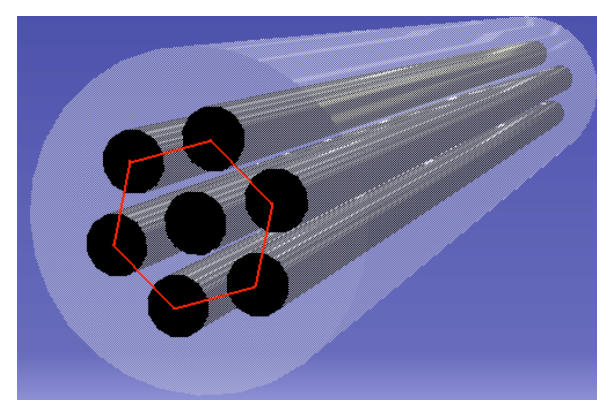
\includegraphics[scale=0.7]{Figures/cluster.eps} 
\caption{Simplified cluster geometry used for CANDU reactor cases.}\label{fig:Cluster}
  \end{center}
\end{figure}

\item[\moc{RADIUS}] keyword used to set the pin-cell radii.

\item[\dusa{r1}] real value set to the fuel pellet radius in m.

\item[\dusa{r2}] real value set to the internal clad rod radius in m.

\item[\dusa{r3}] real value set to the external clad rod radius in m.

\item[\dusa{r4}] real value set to the guide tube radius in m.

\item[\moc{POROS}] keyword used to set the oxyde porosity of fuel. Porosity affects some built-in correlations
used to represent the heat conduction phenomenon in fuel.

\item[\dusa{poros}] real value set to the oxyde porosity. The default value is 0.05.

\item[\moc{PUFR}] keyword used to set the plutonium mass enrichment of fuel. Plutonium enrichment affects some built-in correlations
used to represent the heat conduction phenomenon in fuel.

\item[\dusa{pufr}] real value set to the plutonium mass enrichment. This value can be unique or channel-dependent. The default value is 0.0.

\item[\moc{F-RUG}] keyword used to set the rugosity of the fuel rod, used in M\"uller-Steinhagen correlation for coolant friction.

\item[\dusa{epsr}] real value set to the rugosity of the fuel rod in m. The default value is 0.0.

\item[\moc{THETA}] keyword used to set the angle of the fuel channel, used in M\"uller-Steinhagen correlation for coolant friction.

\item[\dusa{theta}] real value set to the angle of the fuel channel in radians. The default value is 0.0, corresponding to a vertical channel.

\item[\moc{CONDF}] keyword used to set the fuel thermal conductivity as a function of local fuel temperature $T_{fuel}$.
Fuel conductivity is computed as

$$\lambda_{fuel} = \sum_{k=0}^{\dusa{ncond}} {\dusa{kcond}(k)*(T_{fuel})^k + \frac{\dusa{inv}}{T_{fuel}-\dusa{ref}}}$$

with $\lambda_{fuel}$ in $W/m/K$ and $T_{fuel}$ in the selected unit (Kelvin or Celsius).

By default, built-in models are used, taking into account oxyde porosity and plutonium mass enrichment.
Note that oxyde porosity and plutonium mass enrichment are ignored if this keyword is used.

\item[\dusa{ncond}] integer value set to the degree of the conductivity polynomial.

\item[\dusa{kcond}] real value set to the coefficient of the conductivity polynomial. $\dusa{ncond}+1$ coefficients are expected.

\item[\dusa{unit}] string value set to the unit of temperature $T$ in the conductivity function. Can be either \dusa{CELSIUS} or \dusa{KELVIN}.

\item[\moc{INV}] keyword used to add an inverse term in the fuel conductivity function.

\item[\dusa{inv}] real value set to the coefficient in the inverse term of fuel conductivity.
The default value is 0.0 (i.e. no inverse term).

\item[\dusa{ref}] real value set to the reference in the inverse term of fuel conductivity.

\item[\moc{CONDC}] keyword used to set the clad thermal conductivity as a function of local clad temperature $T_{clad}$.
Clad conductivity is computed with the following polynomial

$$\lambda_{clad} = \sum_{k=0}^{\dusa{ncond}} {\dusa{kcond}(k)*(T_{clad})^k}$$

with $\lambda_{clad}$ in $W/m/K$ and $T_{clad}$ in the selected unit (Kelvin or Celsius).

By default, a built-in model is used.

\item[\moc{HGAP}] keyword used to set the heat exchange coefficient of the gap as a constant.
By default, a built-in model is used.

\item[\dusa{hgap}] real value set to the constant heat exchange coefficient of the gap in $W/m^2/K$.

\item[\moc{HCONV}] keyword used to set the heat transfer coefficient between clad and fluid as a constant.
By default, this coefficient is computed using a built-in correlation.

\item[\dusa{hconv}] real value set to the constant heat transfer coefficient between clad and fluid in $W/m^2/K$.

\item[\moc{TEFF}] keyword used to set the weighting factor in the effective fuel temperature approximation.
The effective fuel temperature is used for the cross sections interpolations on fuel temperature.

\item[\dusa{wteff}] real value $W_{\rm teff}$ set to the weighting factor in the effective fuel temperature.
The effective fuel temperature is computed as

$$
T^{\rm fuel}_{\rm eff}=W_{\rm teff}*T^{\rm fuel}_{\rm surface}+(1-W_{\rm teff})*T^{\rm fuel}_{\rm center}
$$

where $0\le W_{\rm teff} \le 1$, $T^{\rm fuel}_{\rm surface}$ is the temperature at the surface of the fuel pellet (K), and $T^{\rm fuel}_{\rm center}$ is the temperature at the center of the fuel pellet (K).

By default, the Rowlands weighting factor $W_{\rm teff}={5 \over 9}$ is used\cite{Rowlands}.

\item[\moc{CONV}] keyword used to set the convergence criteria for solving the conduction and the conservation equation.

\item[\dusa{maxit1}] integer value set to the maximum number of iterations for computing the
conduction integral. The default value is 50.

\item[\dusa{maxit2}] integer value set to the maximum number of iterations for computing the
center pellet temperature. The default value is 50.

\item[\dusa{maxit3}] integer value set to the maximum number of iterations for computing the
coolant parameters (mass flux, pressure, enthalpy and density) in case of a transient calculation. The default value is 50.

\item[\dusa{ermaxt}] real value set to the maximum temperature error in K. The default value is 1~K.

\item[\dusa{ermaxc}] real value set to the maximum relative  error for parameters given by the resolution of flow conservation equations (pressure, velocity and enthalpy). The default value is $10^{-3}$.

\item[\moc{RODMESH}] keyword used to set the radial discretization of pin-cells.

\item[\dusa{nb1}] integer value set to the number of discretisation points in fuel. The default value
is 5.

\item[\dusa{nb2}] integer value set to the number of discretisation points in the whole pin-cell (fuel+cladding). The default value
is 8.

\item[\moc{FORCEAVE}] keyword used to force the use of the average approximation during the fuel conductivity evaluation.
By default, a rectangle quadrature approximation is used.

\item[\moc{MONO}] keyword used to set a one-phase flow model.

\item[\moc{BOWR}] keyword used to set a subcooling model based on the Bowring correlation\cite{bowring} (default option).

\item[\moc{SAHA}] keyword used to set a subcooling model based on the Saha-Zuber correlation\cite{lahey}. This option is recommended for BWR and CANDU applications.

\item[\moc{RAD-PROF}] keyword used to set radial power form factors. By default, these factors are set to 1.0.

\item[\dusa{rprad}] radius corresponding to a form factor with 0 $\le$ \dusa{rprad} $\le$ \dusa{r1}. This value doesn't need to correspond to a
material limit in the fuel rod.

\item[\dusa{fprad}] radial power form factor corresponding to radius \dusa{rprad}.

\item[\moc{POWER-LAW}] keyword used to define a time-dependent power law in the input. By default, the power is recovered from the fuelmap object \dusa{MAPFL}.

\item[\dusa{tpow}] total power delivered in the reactor in W.

\item[\dusa{ntime}] number of tabulation points for the power law.

\item[\dusa{t(i)}] tabulation abscissa in time (s).

\item[\dusa{pow(i)}] tabulation power factor corresponding to \dusa{t(i)}. The reactor power at time \dusa{t(i)} is given as \dusa{tpow}$\times$\dusa{pow(i)}.

\item[\moc{SET-PARAM}] keyword used to indicate the input (or modification)
of the actual values for a parameter specified using its \dusa{PNAME}.

\item[\moc{PNAME}] keyword used to specify \dusa{PNAME}.

\item[\dusa{PNAME}] \texttt{character*12} name of a parameter.

\item[\dusa{pvalue}] single real value containing the actual
parameter's values. Note that this value will not be checked for consistency
by the module. It is the user responsibility to provide the valid parameter's value
which should be consistent with those recorded in the multicompo or Saphyb database.

\item[\moc{PICK}]  keyword used to recover the temperature variation parameter $R$ in a CLE-2000 variable. This parameter describes the variation of
averaged fuel and coolant temperatures during a time step using the formula
$$ R=\max \left\{{1\over \Delta T_{\rm fuel}} \left|\bar T_{\rm fuel}(n)-\bar T_{\rm fuel}(n-1)\right|,
 {1\over \Delta T_{\rm cool}} \left|\bar T_{\rm cool}(n)-\bar T_{\rm cool}(n-1)\right| \right\}$$

\noindent where $\Delta T_{\rm fuel}=5 \ {\rm K}$ and $\Delta T_{\rm cool}=40 \ {\rm K}$.

\item[\dusa{ratio}] \texttt{character*12} CLE-2000 variable name in which the temperature variation parameter will be placed.

\end{ListeDeDescription}
\clearpage
